\documentclass[a4paper,UTF8]{article}
\usepackage{graphics}
\usepackage{xeCJK}
\usepackage{fancyhdr}
\usepackage{indentfirst}
\usepackage{bigstrut}
\usepackage{multirow}
\usepackage{listings}
\usepackage[framed,numbered,autolinebreaks,useliterate]{mcode}
\usepackage{appendix}
\usepackage{lscape}
\newCJKfontfamily[kaiti]\kaiti{KaiTi}

\newcommand{\yihao}{\fontsize{26pt}{36pt}\selectfont}           % 一号, 1.4 倍行距
\newcommand{\erhao}{\fontsize{22pt}{28pt}\selectfont}          % 二号, 1.25倍行距
\newcommand{\xiaoer}{\fontsize{18pt}{18pt}\selectfont}          % 小二, 单倍行距
\newcommand{\sanhao}{\fontsize{16pt}{24pt}\selectfont}        % 三号, 1.5倍行距
\newcommand{\xiaosan}{\fontsize{15pt}{22pt}\selectfont}        % 小三, 1.5倍行距
\newcommand{\sihao}{\fontsize{14pt}{21pt}\selectfont}            % 四号, 1.5 倍行距
\newcommand{\banxiaosi}{\fontsize{13pt}{19.5pt}\selectfont}    % 半小四, 1.5倍行距
\newcommand{\xiaosi}{\fontsize{12pt}{18pt}\selectfont}            % 小四, 1.5倍行距
\newcommand{\dawuhao}{\fontsize{11pt}{11pt}\selectfont}       % 大五号, 单倍行距
\newcommand{\wuhao}{\fontsize{10.5pt}{15.75pt}\selectfont}    % 五号, 单倍行距

\pagestyle{fancy}
\fancyhf{}
\lhead{
\includegraphics{figure/sjtubanner}}
\chead{}
\rhead{船舶原理2018}%需修改之处
\lfoot{}
\cfoot{\small --~~{\bfseries\thepage}~~of~~{\bfseries{\pageref{last}}}~~--}
\rfoot{}
\fancyheadoffset{50pt}
\renewcommand{\headheight}{32pt}

\setlength{\parindent}{2.45em}%来调整首行缩进的大小。这里的 2.45em 是中文小四号字大小两个中文字的长度。

\begin{document}
\begin{titlepage}
	\thispagestyle{empty}
	\begin{center}
		\vspace*{20pt} \vskip 7pt
		
\includegraphics{figure/sjtulogo}
		\vskip 30pt
		{\kaiti \fontsize{32}{32} 螺旋桨设计}%修改之处
		\vskip 15pt 
		{\xiaosi \MakeUppercase{\textbf{Ship Principle Project--Propeller Desigh}}}%修改之处
		\vskip 15pt
		
\includegraphics[trim=0 0 0 -2cm]{figure/sjtubadge}
		\vskip \stretch{2}
		    \vskip \stretch{1}
		{\kaiti\sanhao
			\def\arraystretch{1.1}
			\begin{tabular}{r@{:}l}%修改之处
				\makebox[4em][s]{学生姓名}        & \underline{\makebox[180pt]{简心语}} \\
				\makebox[4em][s]{学生学号} 		& \underline{\makebox[180pt]{515021910260}} \\
				\makebox[4em][s]{专\hspace{\fill}业}    	      & \underline{\makebox[180pt]{船舶与海洋工程}} \\
				\makebox[4em][s]{指导老师}        & \underline{\makebox[180pt]{杨晨俊}} \\
				\makebox[4em][s]{学\hspace{\fill}院}     & \underline{\makebox[180pt]{船舶海洋与建筑工程学院}}
		\end{tabular}}
	\end{center}
\end{titlepage}

\tableofcontents
\newpage
\section{Introduction}
The goal is to design a MAU right-handed propeller with five blades for a certain container ship.
\section{Data}
\subsection{Main Parameters of the Container Ship}
Table \ref{tab:mp} gives the main parameters of the container ship.\\
\begin{table}[!htbp]
	\centering
	\begin{tabular}{cccc}
		\hline
		$L_{wl}$ & Design waterline  & 215 & $m$ \bigstrut\\
		$L_{pp}$ &Length between perpendiculars & 210 & $m$\bigstrut\\
		$ B$ &Breadth   &  32 & $m$ \bigstrut\\
		$ D $ &Depth &   12.7 & $m$ \bigstrut\\
		$ \Delta$ & Volume of displacement &  54000&$m^3$\bigstrut\\
		$C_b$ & Block coefficient    & 0.655 & - \bigstrut\\
		\hline
	\end{tabular}%
	\caption{Main Parameters}
	\label{tab:mp}%
\end{table}%

The datasheet of the ship's effective power in different speed has been given as Table \ref{tab:ep}.
\begin{table}[htbp]
	\centering
	\begin{tabular}{cccc}
		\hline
		Ship Speed(kn) & Ballast(kW) &Full load(kW) & Super full load(kW) \bigstrut\\
		\hline
		19    & 7542  & 9552  & 11323 \bigstrut\\

		19.5  & 8117  & 10275 & 12186 \bigstrut\\

		20    & 8861  & 11208 & 13303 \bigstrut\\

		20.5  & 9689  & 12247 & 14544 \bigstrut\\

		21    & 10562 & 13342 & 15855 \bigstrut\\

		21.5  & 11490 & 14506 & 17248 \bigstrut\\

		22    & 12532 & 15812 & 18811 \bigstrut\\

		22.5  & 13791 & 17389 & 20700 \bigstrut\\

		23    & 15420 & 19429 & 23143 \bigstrut\\

		23.5  & 17618 & 22181 & 26442 \bigstrut\\

		24    & 20634 & 25954 & 30966 \bigstrut\\

		24.5  & 24762 & 31118 & 37159 \bigstrut\\

		25    & 30345 & 38100 & 45533 \bigstrut\\
		\hline
	\end{tabular}%
    \caption{Effective Power}
	\label{tab:ep}%
\end{table}%

\subsection{Parameters of Main Engine and Propeller}
Parameters of main engine and propeller are shown in Tab. \ref{tab:mep}.
\begin{table}
	\centering
	\begin{tabular}{cccc}
		\hline
		$MCR$ & maximum continuous rating of main engine & 33000 & kW\\
		N  &  rated speed & 102 & rpm\\
		- & type of the propeller & MAU series & -\\
		n & number of the blades & 5 & -\\
		- & number of the propeller & 1 &-\\
		- & direction of the propeller & right-handed & -\\
		- & material of the propeller & Cu3 nickel aluminum bronze & -\\
		$Z_p$ & distance between the boss and the base line & 4.7 & m\\
		$d_h$ & diameter of the boss & 1.4 &m\\
		\hline 
	\end{tabular}
	\caption{Main Engine and Propeller}
	\label{tab:mep}
\end{table}
\subsection{Design Conditions}
 \begin{table}[!htbp]
 	\centering
 	\begin{tabular}{cc}
 		\hline
		 design condition & full load \\
		 design main engine power & $P_s=0.85MCR=28050kw$\\
		 desing rotating speed & $N=102rpm$\\
		 \hline
 	\end{tabular}
 	\caption{Design Conditions}
 \end{table}

\subsection{Propulsive Factors}
\begin{table}[!htbp]
	\centering
	\begin{tabular}{ccc}
		\hline
		$\omega$ & wake fraction & 0.25\\
		$t$		& thrust deduction fraction & 0.16\\
		$\eta_R$ & relative rotating efficiency & 1.0 \\
		$\eta_s$ & shaft system efficiency & 0.98\\
		$\eta_H$ & ship hull efficiency & 1.12\\
		\hline
	\end{tabular}
\caption{Propulsive Factors}
\end{table}

\section{Design for Maximum Ship Speed}
In this part, we select a number of EARs(Extend Area Ratio), and determine a maximum ship speed for each of them.\\

\subsection{Related Parameters}
Firstly, the basic related parameters is shown in Tab \ref{tab:rp}.
\begin{table}
	\centering
	\begin{tabular}{lc}
		\hline
		density of sea water($15^{\circ}C$)&$\rho=1025.91kg/m^3=104.63kgf\cdot s^2/m^4$\\
		main engine power &  $P_s=0.85MCR=28050kw$\\
		receiveing power of propeller in open water & $P_D=\eta_s\eta_RP_s=27209kW$\\
		rotating speed of propeller & N=102rpm=1.7rps\\
		receiveing torque of propeller & $Q=\frac{P_D}{2\pi n}=2.547\time 10^6N\cdot m$\\
		\hline
	\end{tabular}
	\caption{Related Parameters in Speed Design}
	\label{tab:rp}
\end{table}

\subsection{Assume Parameters}
\begin{enumerate}
	\item In the range of 0.5 to 0.8, we assume 7 EARs in equivilent distance.
	\item For each EAR, assuming 21 diameters between 7.5m to 8.5m in the step of 0.05m. 
	\item For each diameter, assuming 21 crusing speed between 21kn to 25kn in the step of 0.2.
	\item For each diameter, assuming 13 pitch ratios between 0.4 to 1.6 in the step of 0.1.
	\item According to the torque equilibrium and using the regression formula, we can get different thrusts and torques in different pitch ratios for each diameter and cruising speed. Furthermore, we can get the right pitch ratio, the effective thrust and the open water efficiency using interpolation.
	\item We can determine the cruising speed by interpolation when the effective thrust equals to the drag force for each diameter. Thus, the pitch ration can be set.
	\item Choosing the maximum opening water efficiency,we can get the diameter accordingly.
\end{enumerate}
We can do caculation in Matlab following the procedure above. The code is shown in Appendix. The result is in the Tab. \ref{tab:fact}.
\begin{table}[!htbp]
	\centering

	\begin{tabular}{cccc}
		\hline
		EAR & Diameter & Crusing Speed & Pitch Ratio \\
$\frac{A_E}{A_0}$     &   D    &   $V_s$    & $\frac{P}{D}$ \\
\hline
0.50  & 7.7406  & 23.9632  & 0.9380  \\
0.55  & 7.8925  & 23.9861  & 0.9087  \\
0.60  & 7.6945  & 24.0030  & 0.9675  \\
0.65  & 8.0147  & 24.0056  & 0.8948  \\
0.70  & 7.8520  & 23.9855  & 0.9381  \\
0.75  & 7.8476  & 23.9347  & 0.9392  \\
0.80  & 8.1915  & 23.8449  & 0.8474  \\
\hline
Advance Coefficient&Thrust Coefficient&Torque Coefficient&Open Water Efficiency \\
J&$K_t$&$K_q$&$\eta_0$\\
\hline
0.6457  & 0.1865  & 0.0309  & 0.7020  \\
0.8643  & 0.1736  & 0.0280  & 0.6891  \\
0.7365  & 0.1923  & 0.0316  & 0.7070  \\
0.7062  & 0.1638  & 0.0259  & 0.6790  \\
0.7166  & 0.1773  & 0.0288  & 0.6927  \\
0.7167  & 0.1749  & 0.0288  & 0.6916  \\
0.8297  & 0.1363  & 0.0214  & 0.6571  \\
		\hline
	\end{tabular}%
	\caption{Best Parameters for Design}
	\label{tab:fact}%
\end{table}%

\section{Cavitation Check}
Determine an EAR required for each propeller design to be cavitation-
free, and subsequently determine the minimum EAR that ensures the
propeller has the highest efficiency while being free of cavitation. 
\subsection{Related Parameters}
\begin{table}[!htbp]
	\centering
	\begin{tabular}{cc}
	\hline
	Depth of the boss & $h_s=D-Z_p=8m$\\
	wake fraction &$\omega=0.25$\\
	\hline
	Sea water mass density($15^{\circ}C$)&$\rho=104.63kgf\cdot s^2/m^4$\\
	Sea water gravity density($15^{\circ}C$)&$\gamma=1025.91kg/m^3$\\
	Sea water vapor pressure($15^{\circ}C$)&$p_v=174kgf/m^2$\\
	Atmospheric pressure($15^{\circ}C$)&$p_a=10330kg/m^2$\\
	\hline
	\end{tabular}
	\caption{Basic Parameters}
\end{table}
Thus, we can caculate the differential pressure conditions:
\begin{equation}
	p_0-p_v=p_a+\gamma h_s-p_v=10330+1025.91×8−174 = 18363.28kgf/m^2
\end{equation}
The principle equations are as follows:\\
\begin{equation}
\centering
\left\{
\begin{array}{lr}
\sigma_{0.7R}=\frac{P_0-P_v}{\frac{1}{2}\rho V_{0.7R}^2} \\
\tau=\frac{T/AP}{\frac{1}{2}\rho V_{0.7R}^2} 
\end{array}
\right.
\label{equ:kongpao}
\end{equation}

In this part, it is convenient to use EXCEL and caculation sheet is shown in Appendix. The cavitation verification results are shown in Tab.\ref{tab:cavitation}.
\begin{table}[!htbp]
	\centering
	\begin{tabular}{ccccccccc}
		\hline
		&       & \multicolumn{1}{l}{MAU5-50} & \multicolumn{1}{l}{MAU5-55} & \multicolumn{1}{l}{MAU5-60} & \multicolumn{1}{l}{MAU5-65} & \multicolumn{1}{l}{MAU5-70} & \multicolumn{1}{l}{MAU5-75} & \multicolumn{1}{l}{MAU5-80} \\
		$V_max$  & kn    & 23.9632  & 23.9861  & 24.0030  & 24.0056  & 23.9855  & 23.9347  & 23.8449  \\
		D & m     & 7.7406  & 7.8925  & 7.6945  & 8.0147  & 7.8520  & 7.8476  & 8.1915  \\
		$\eta_0$ & -     & 0.7020  & 0.6891  & 0.7070  & 0.6790  & 0.6927  & 0.6916  & 0.6571  \\
		$V^2_{0.7R}$ & $m/s\^2$ & 922.8968 & 956.2511 & 913.2449 & 983.5733 & 947.3309 & 946.0171 & 1022.459 \\
		$\sigma_{0.7R}$  & -     & 0.3803  & 0.3671  & 0.3844  & 0.3569  & 0.3705  & 0.3710  & 0.3433  \\
		$\tau_c$ & -     & 0.1481 & 0.1425 & 0.1484 & 0.1393 & 0.1437 & 0.1439 & 0.1372 \\
		$P/D$ & -     & 0.9380  & 0.9087  & 0.9675  & 0.8948  & 0.9381  & 0.9392  & 0.8474  \\
		$A_E/A_0$ & -     & 0.7422  & 0.6968  & 0.7678  & 0.6592  & 0.7140  & 0.7153  & 0.5930  \\
		\hline
	\end{tabular}
	\caption{Cavitation Check Results}
	\label{tab:cavitation}
\end{table}
According to the result of EAR above, we can get the Fig.\ref{fig:cavitation}. From the figure, the point of intersection of two curves is the EAR we want, which satisfies the conditions of maximum crusing speed, thrust equivalence. Meanwhile, we can get the minimum extend area ratio when there is no cavitation through interpolation. Furthermore, other best propeller factors can be achieved. The result is shown in Tab.\ref{tab:cavicheck}
\begin{figure}
	\centering
	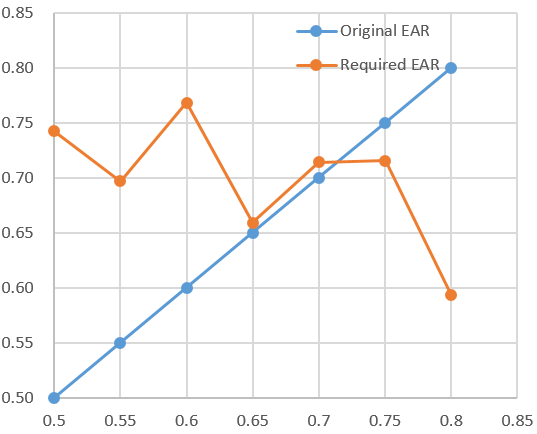
\includegraphics[width=3in]{figure/cavitation_check.png}
	\caption{Cavitation Checking Result}
	\label{fig:cavitation}
\end{figure}
\begin{table}[!htbp]
	\centering
	\begin{tabular}{ccc}
		\hline
		Extend Area Ration(EAR)&$A_E/A_0$&0.7145\\
		Maximum Speed&$V_max$&23.9601kn\\
		Diameter&D&7.8498m\\
		Pitch Ratio&$P/D$&0.9386 \\ 
		Open Water Efficiency&$\eta_0$&0.6921 \\
		\hline
	\end{tabular}	
	\caption{Best Parameters of Propeller}
	\label{tab:cavicheck}
\end{table}

\section{Strength Check}
Safty is one of the most important issues among the design.Aaccording to the principle of the "Rules and Regulations for the Construction and Classification of Sea Going Steel Ships" in 2001, we should check the $t_{0.25R}$ and $t_{0.6R}$ whether they are both bigger than the following value:
\begin{equation}
	t=\sqrt{\frac{Y}{K-X}}
\end{equation}
Specifically, X is called rotate speed coefficient and Y is called power coefficient, $K=1.38$ is material factor of Cu3 nickel aluminum bronze.

\subsection{Power Coefficient}
\begin{equation}
		Y=\frac{1.36A_1N_e}{Zbn_e}
\end{equation}

\begin{equation}
	A_1=\frac{D}{P}(K_1-K_2\frac{D}{P_{0.7}})+K_3\frac{D}{P_{0.7}}-K_4
\end{equation}

The diameter of the propeller: $D=7.8498m$\\
The pitch ratio in the section: $P=P_{0.7}=\frac{P}{D}D=0.9386\times7.8498=7.3678$\\
$K_1-K_4$ can be found in Tab.\ref{tab:k}\\
The main engine power: $N_e=32010kw=43551hp$\\
The number of blades: $Z=5$\\
The rotating speed of propeller: $n_e=102rpm$\\
According to the blades outline of the AU propeller, we can calculate the b:
\begin{equation}
	b_{0.66R}=0.266D\frac{EAR}{0.1Z}=2.9838m
\end{equation}
$b_{0.25R}=0.7212b_{0.66R}=2.1519m$,$b_{0.6R}=0.9911b_{0.66R}=2.9573m$.
\begin{table}[htbp]
	\centering
	\begin{tabular}{ccccccccc}
	\hline
	Radius & $K_1$ & $K_2$ &$K_3$  & $K_4$ &$K_5$  & $K_6$ & $K_7$&$K_8$ \\
	0.25R& 634   & 250   & 1410  & 4     & 82    & 34    & 41    & 380 \\
	0.60R& 207   & 151   & 635   & 34    & 23    & 12    & 65    & 330 \\
	\hline
	\end{tabular}
	\caption{K Factor Table of Different Radius of Propeller}
	\label{tab:k}
\end{table}

\subsection{Rotate Speed Coefficient}
\begin{equation}
		X=\frac{A_2GA_dN^2D^3}{10^{10}Zb}
\end{equation}
\begin{equation}
		A_2 = \frac{D}{P}(K_5 + K_6\epsilon) + K_7\epsilon + K_8
\end{equation}
$D,P,n_e,Z,b$ are the same with Y.\\
The back-inclined angle: $\epsilon=10^\circ$\\
The density of blades: $G=7.6g\cdot cm^{-3}$\\
The extend area ratio: $A_d=0.7145$ \\
$K_5-K_8$ can be found in Tab.\ref{tab:k}\\
Results of caculation of cavitation varification are shown in Tab.\ref{tab:strcheck}.

\begin{table}[!htbp]
	\centering
	\begin{tabular}{p{3cm}ccc}
		\hline
		    &  & \multicolumn{1}{l}{0.25R} & \multicolumn{1}{l}{0.6R} \\
		b   & 	m	 & 2.1519 & 2.9573 \\
		A1    &       & 1925.033 & 703.7262 \\
		Y     &       & 76360.82 & 20312.47 \\
		A2    &       & 1249.445 & 1135.689 \\
		X     &       & 0.317334 & 0.209887 \\
		t     &	mm  & 268.063 & 131.7551 \\
		Standard & mm & 300.2549 & 171.1256 \\
		Checking Results  &       & Satisfied & Satisfied \\
		\hline
	\end{tabular}
	\caption{Strength checking}
	\label{tab:strcheck}
\end{table}
As a result, we can determine the propeller’s thickness in different radiuses as Tab.\ref{tab:jiangyehoudu} shows.
\begin{table}[!htbp]
	\centering
	\begin{tabular}{llllllllll}
		\hline
		$r/R$  & 0.2        & 0.3        & 0.4        & 0.5        & 0.6        & 0.7        & 0.8        & 0.9        & 1.0       \\
		\hline
		$t/mm$ & 324.6  & 287.4  & 250.3  & 213.2  & 176.0  & 138.9  & 101.7  & 64.6  & 27.5  \\
		\hline
	\end{tabular}
	\caption{The Propeller’s Thickness in Different Radiuses}
	\label{tab:jiangyehoudu}
\end{table}

\section{Pitch Ratio Modification}
\subsection{Different Hub to Diameter Ratios}
MAU series five blades propeller's standard pitch ratio is 0.18. However, according to design, the ratio is $(\frac{d_h}{D})^\prime=\frac{1.4}{7.8498}=0.1783$. Thus, modification is needed.
\begin{equation}
\centering
\Delta\left(\frac{d_h}{D}\right)_b=\frac{1}{10}[(\frac{d_h}{D})^\prime-(\frac{d_h}{D})]=-0.000165
\end{equation}
\subsection{Different Blade Thickness Ratios}
Because MAU series propeller's thickness fail to pass the strength varification, another modification is needed. Setting MAU5-80 as standard propeller to modifiy.\\
Standard Propeller $(\frac{t}{b})_{0.7R}=0.04715$\\
\qquad $a_E=0.8$\\
Real Propeller $(\frac{t}{b})^\prime_{0.7R}=0.05498$\\
\qquad $a_E^\prime = (1+1.1[(\frac{d_h}{D})^\prime-(\frac{d_h}{D})])\frac{A_E}{A_0}=0.7132$\\
\begin{equation}
\Delta(\frac{t}{b})_{0.7R} =[ (\frac{t}{b})'_{0.7R} - (\frac{t}{b})_{0.7R}\times\frac{a_E}{a_E^\prime}]\times 0.75 = 0.001569
\end{equation}

\begin{equation}
1-s = \frac{V_A}{NP} = \frac{30.866(1-w)V}{NP} =0.6927
\end{equation}

\begin{equation}
\Delta (\frac{P}{D})_t = -2\frac{P}{D}(1-s)\Delta(\frac{t}{b})_{0.7R} = -0.00204
\end{equation}

\subsection{Final Pitch Ratio}
\begin{equation}
(\frac{P}{D})_m = \frac{P}{D} + \Delta(\frac{P}{D})_B + \Delta(\frac{P}{D})_t =0.9364
\end{equation}


\section{Calculation of Weight and Inertia Moment}
\subsection{The Weight and Length}
The weight of the blades:
\begin{equation}
G_{b1}=0.169\gamma Zb_{max}\left(0.5t_{0.2R}+t_{0.6R}\right)\left(1-\frac{d}{D}\right)D=41810.7788kgf
\end{equation}

The length of the hub: $L_K=0.2D=1.5699m$\\
The weight of the hub:
\begin{equation}
G_n=\left(0.88-0.6\frac{d_0}{d}\right)l_K\gamma d^2=12743.1 kgf
\end{equation}

\begin{equation}
d_0=0.045+0.108\left(\frac{P_D}{N}\right)^{1/3}-\frac{KL_K}{2}=0.78535
\end{equation}
Thus, the overall weight of the propeller $G=G_{b1}+G_n=54553.9kgf$
The value of related parameters are given in Tab.\ref{tab:weightlength}.
\begin{table}[!htbp]
	\centering
	\begin{tabular}{cccc}
		\hline
		$\gamma$ & $7600kgf/m^3$ & Z & 5\\
		$b_max=b_{0.66R}$  & 2.9838m & d & 1.4m\\
		$t_{0.2R}$ & 324.6mm & $t_{0.6R}$ & 176mm\\
		D & 7.8498m & $P_D$ &43970.1hp \\
		N & 102rpm & K & $\frac{1}{10}$ \\
		\hline
	\end{tabular}
	\caption{Related Parameters of Weight and Length}
	\label{tab:weightlength}
\end{table}

\subsection{Inertia}
First, we caculate:
\begin{equation}
\frac{d}{D}=\frac{d_h}{D}=\frac{1.4}{7.8498}=0.1783 \leq 0.18
\end{equation}
Thus, we can get:\\
\begin{equation}
I_{mp}=0.0948\gamma Zb_{max}\left(0.5t_{0.2}+t_{0.6}\right)D^3=1758892.985kgf\cdot cm\cdot s^2
\end{equation}

\section{Open Water Graph of Propeller}
Considering propeller open water characteristics regression curve formula:
\begin{equation}
\left\{
\begin{array}{lr}
K_T=\sum_{k=1}^{16}a_k\left(\frac{A_E}{A_0}\right)^{r_k}\left(\frac{P}{D}\right)^{s_k}J^{t_k} \\
10K_Q=\sum_{k=1}^{23}b_k\left(\frac{A_E}{A_0}\right)^{u_k}\left(\frac{P}{D}\right)^{v_k}J^{w_k} \\
\eta_0=\frac{K_T}{K_Q}\frac{J}{2\pi}
\end{array}
\right.
\end{equation}
Related parameters are Extend Area Ratio $\frac{A_E}{A_0}=0.7145$ and Pitch Ratio $\frac{P}{D}=0.9364$. Now we can draw curves as Fig.\ref{fig:changshui} shows.\\
\begin{figure}
	\centering
	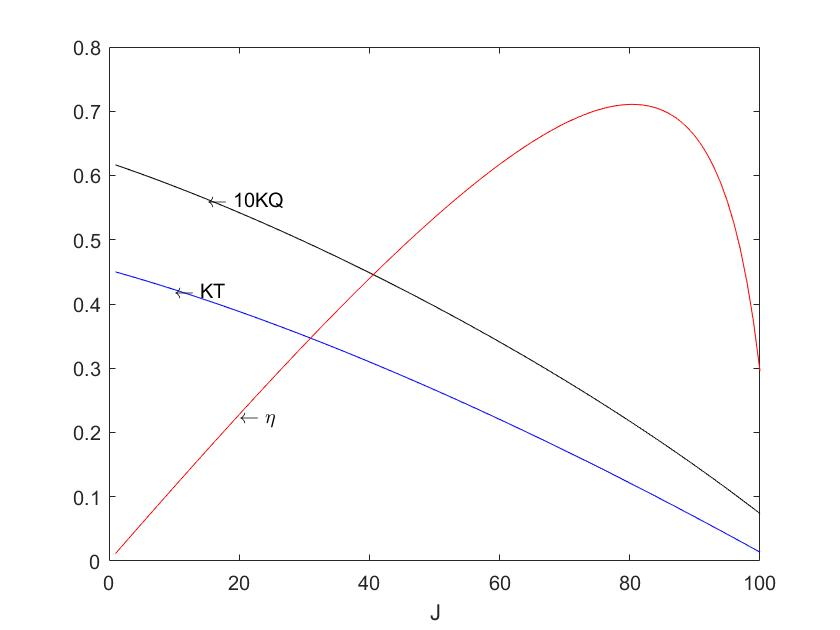
\includegraphics[width=4in]{figure/changshui.jpg}
	\caption{Open Water Graph}
	\label{fig:changshui}
\end{figure}

\section{Calculation of the Tied Column}
From open water graph, we can get $K_T,K_Q$ when J=0 and do caculations. The result is shown in Tab.\ref{tab:xizhu}.
\begin{table}[h]
	\centering

	\begin{tabular}{lll}
		\hline
		J      &     & 0           \\
		$K_T$     &     & 0.4529       \\
		$K_Q$     &     & 0.62     \\
  		  D     & m     & 7.8498 \\
	power & KW    & 32340 \\
	 tied column thrust deduction fraction &       & 0.04 \\
main engine torque  & N·m   & 3027688.741 \\
tied column thrust  & N     & 281749.5722 \\
rotating speed of the propeller  & r/s   & 0.399807886 \\
		\hline
	\end{tabular}
	\caption{Tied Column Characteristics}
	\label{tab:xizhu}
\end{table}

\section{Calculation of the Cruising Characters}
When the rotating speed equals to 102rpm, 97rpm, 92rpm, we can get the following results as Tab.\ref{tab:hangxingtexing} shows and draw Fig.\ref{fig:hangxing}.

\begin{table}[htbp]

	\begin{tabular}{clrrrrr}
		\hline
		\multicolumn{2}{c}{Speed} & 21    & 22    & 23    & 24    & 25 \\
		\hline
		\multicolumn{2}{c}{Advance Speed} & 8.1025  & 8.4883  & 8.8741  & 9.2600  & 9.6458  \\
		\multicolumn{2}{c}{Diameter} & 7.8498  & 7.8498  & 7.8498  & 7.8498  & 7.8498  \\
		\multicolumn{2}{c}{Pitch Ratio} & 0.9364  & 0.9364  & 0.9364  & 0.9364  & 0.9364  \\
		\hline
		\multirow{5}[0]{*}{102} & J     & 0.6072  & 0.6361  & 0.6650  & 0.6939  & 0.7228  \\
		& KT    & 0.2170  & 0.2032  & 0.1892  & 0.1750  & 0.1607  \\
		& KQ    & 0.0337  & 0.0320  & 0.0303  & 0.0285  & 0.0267  \\
		& Effective Power & 22151.6100  & 21730.3294  & 21153.3168  & 20418.1316  & 19522.3492  \\
		& Main Engine Power & 32413.6127  & 30788.6961  & 29131.4690  & 27440.8480  & 25715.6250  \\
		\hline
		\multirow{5}[0]{*}{95} & J     & 0.6519  & 0.6830  & 0.7140  & 0.7450  & 0.7761  \\
		& KT    & 0.1956  & 0.1804  & 0.1651  & 0.1495  & 0.1337  \\
		& KQ    & 0.0311  & 0.0292  & 0.0273  & 0.0253  & 0.0233  \\
		& Effective Power & 17316.9855  & 16736.5377  & 16007.3687  & 15127.0594  & 14093.1918  \\
		& Main Engine Power & 24145.3232  & 22690.9451  & 21204.7782  & 19685.5318  & 18131.7809  \\
		\hline
		\multirow{5}[0]{*}{85} & J     & 0.7286  & 0.7633  & 0.7980  & 0.8327  & 0.8674  \\
		& KT    & 0.1578  & 0.1402  & 0.1224  & 0.1044  & 0.0861  \\
		& KQ    & 0.0264  & 0.0241  & 0.0219  & 0.0196  & 0.0172  \\
		& Effective Power & 11182.7016  & 10413.1062  & 9504.8403  & 8455.4640  & 7262.5075  \\
		& Main Engine Power & 14679.5793  & 13448.8532  & 12186.4460  & 10890.7113  & 9559.8528  \\
		\hline
	\end{tabular}%
	\caption{Cruising Results of the Ship}
	\label{tab:hangxingtexing}
\end{table}
\begin{figure}[!htbp]
	\centering
	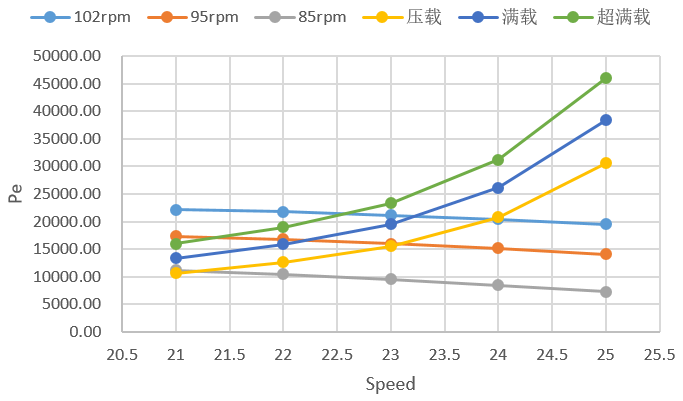
\includegraphics[width=5in]{figure/hangxingtexing.png}
	\caption{Cruising Characteristics Graph}
	\label{fig:hangxing}
\end{figure}
According to the caculation results, we can get the maximum crusing speed and power of the main engine by interpolation as Tab.\ref{tab:final} shows.
\begin{table}[!htbp]
	\centering
	\begin{tabular}{ccc}
		\hline
		Cruising Condition & Maximum Cruising Speed)(kn) & Power of Main Engine(w)\\
		Ballast&23.94&27546.97\\
		Fully Loaded&23.22&28759.24 \\
		Super Fully Loaded &22.56&	29868.74\\
		\hline
	\end{tabular}
\caption{Final Results}
\label{tab:final}
\end{table}

\section{Conclusion}
Now, we have the ultimate design of the propeller. The data is shown in Tab.\ref{tab:conclusion}.

\begin{table}[htbp]
	\centering
	\begin{tabular}{cccc}
		\hline
		Diameter & \textit{D} & 7.8498   & \textit{m}\\
		Pitch Ratio & \textit{P/D} & 0.9364  & - \\
		Type  &  & MAU &  \\
		Number of Blades & \textit{Z} & 5     &- \\
		EAR   & $A_E/A_0$ & 0.7145 & - \\
		Inclined Angle & $\epsilon$ & 10    & \textit{degree} \\
		Open Water Efficiency & $\eta_0 $ & 0.6921 & - \\
		Designed Cruising Speed & V     & 23.9601  & \textit{kn} \\
		Ratio of boss to diameter & $d_h/D$  & 0.1783 & - \\
		Rotating Direction &  & Right & - \\
		Material & & Cu3 nickle  aluminum bronze & - \\
		Weight & G     & 54553.9 & \textit{kgf} \\
		Inertial Moment & I & 1758892.985 & $kgf·cm·s^2$\\
		\hline
	\end{tabular}%
	\caption{Ultimate Design}
	\label{tab:conclusion}%
\end{table}%

\begin{appendices}
	\section{Code}
	\begin{lstlisting}[language={Matlab},caption={Caculate Max Speed}]
	%初始化参数
	n=1.7;  %螺旋桨转速rps
	w=0.25; %伴流系数
	t=0.16; %推力减额分数
	% Pmax=33000000; %主机最大持续功率 W
	% PS=0.85*Pmax;  %主机功率 W
	% P_D=0.98*1*PS; %螺旋桨敞水收到功率 W
	Q=2.547E6;       %螺旋桨收到转矩
	den=1025.91;   %海水密度 kg/m^3
	Result=zeros(40131,8); %
	k=0;
	%%------------最大航速计算------------%%
	%计算出每种组合对应的kt,kq,eff
	for EAR=0.5:0.05:0.8 %伸张面比 7个
	for D=7.5:0.05:8.5 %直径 21个
	for Vs=21:0.2:25 %航速 21个
	for m=1:13
	PD=0.1*m+0.3;%螺距比 pitch ratio 共13个
	J=0.5144*(1-w)*Vs/(n*D); %计算进速系数J
	[Kt, Kq]=calKtKq(J, EAR, PD);%计算推力系数Kt,转矩系数Kq
	eta0 = (Kt./Kq)*(J/(2*pi));   %计算敞水效率eta0
	Result(m+k,1)=EAR;      %计算结果矩阵第一列是伸张面比
	Result(m+k,2)=D;        %第二列是直径
	Result(m+k,3)=Vs;       %第三列是航速
	Result(m+k,4)=J;        %第四列是进速系数
	Result(m+k,5)=PD;       %第五列是螺距比
	Result(m+k,6)=Kt;       %第六列是推力系数
	Result(m+k,7)=Kq;       %第七列是转矩系数
	Result(m+k,8)=eta0;     %第八列是敞水效率
	end
	k=k+13;
	end
	end
	end
	
	%%-------通过插值确定满足设计功率要求(即:螺旋桨要求的扭矩与设计功率
	%%与转速下的收到转矩平衡)的螺距及相应的有效推力与敞水效率)--------%%
	PD_req = findPD(Result, Q, den, n);
	
	%%--------对每个直径,根据阻力曲线及不同航速下的有效推力值,通过插值
	%%确定有效推力与阻力平衡的航速,以及对应的螺距和敞水效率----------%%
	Vs_req = findVs(PD_req,den,n,w,t);
	output = findD(Vs_req);
	
	
	function [Kt,Kq]= calKtKq(J, EAR, PD)
	%计算推力系数(Thrust Coefficient)Kt,转矩系数(Torque Coe.)Kq
	%输入:进速系数(Advance Coe.)J, 伸张面比(Extend Area Ratio)EAR, 螺距比(Pitch Ratio)PD
	%输出:推力系数(Thrust Coefficient)Kt,转矩系数(Torque Coe.)Kq
	a=[0.05367018,-0.3023566,0.4333625,-0.1065471,-0.6582904,0.1189101, ...
	-0.0004408557,-0.03317857,1.151124,0.1960773,-0.09747062,0.2036384, ...
	-0.2566153,-0.1370242,-0.2874294,-0.2851609];
	r=[0,0,0,1,3,1,0,1,2,3,1,0,1,0,2,1];
	s=[0,0,1,0,2,1,6,1,2,0,3,1,1,0,0,2];
	t=[0,1,0,2,0,3,0,4,0,0,0,1,1,2,0,0];
	b=[-0.0925139,-0.1229,0.3050697,-0.2935303,-0.3991474,-1.02205,...
	0.01022833,0.0035211,0.002552059,0.2143532,0.000713111,0.2078488,...
	0.6397058,0.0009404846,-0.02930044,-0.07807623,-0.3025523,0.1855105,...
	-0.672421,-0.2087142,0.9400654,0.9316346,-0.04348397];
	u=[0,0,0,0,1,1,0,3,0,3,0,1,0,0,1,0,3,1,2,3,1,3,0];
	v=[0,2,1,0,2,1,7,1,5,0,4,1,1,7,0,0,2,1,2,4,3,2,6];
	w=[0,0,1,2,0,1,0,0,2,1,4,2,0,1,1,4,2,3,1,0,0,1,0];
	Kt=0;
	Kq=0;
	for i=1:16
	Kt=Kt+a(i)*(EAR)^(r(i))*(PD)^(s(i))*(J)^(t(i));
	end
	for i=1:23
	Kq=Kq+(b(i)*(EAR)^(u(i))*(PD)^(v(i))*(J)^(w(i)))/10;
	end
	
	function PD_req = findPD(Result, Q, den, n)
	%在某个螺旋桨直径下, 通过插值确定满足设计功率要求(即:螺旋桨
	%要求的扭矩与设计功率与转速下的收到转矩平衡)的螺距及相应的有效推力
	%与敞水效率)
	%输入:Result
	%     螺旋桨收到转矩D, 海水密度den, 螺旋桨转速n
	%输出:每个螺旋桨直径下合适的螺距比PD
	k=1;
	PD_req=zeros(length(Result)/13,8);
	for i=1:1:length(Result)/13
	Kq_req=Q/(den*n^2*Result(k,2)^5);%螺旋桨要求的扭矩
	PD_req(i,1)=Result(k,1);%固定盘面比
	PD_req(i,2)=Result(k,2);%固定直径
	PD_req(i,3)=Result(k,3);%固定航速
	%由扭矩系数插值得到螺距比
	PD_req(i,4)=interp1(Result(k:k+12,7),Result(k:k+12,5),Kq_req,'spline');
	%由扭矩系数插值得到敞水效率
	PD_req(i,5)=interp1(Result(k:k+12,7),Result(k:k+12,8),Kq_req,'spline');
	%由扭矩系数插值得到推力系数
	PD_req(i,6)=interp1(Result(k:k+12,7),Result(k:k+12,6),Kq_req,'spline');
	%由推力系数计算出的有效推力
	PD_req(i,7)=PD_req(i,6)*den*n^2*Result(k,2)^4;
	PD_req(i,8)=Kq_req;%对应扭矩系数
	k=k+13;
	end
	
	function Vs_req = findVs(PD_req,den,n,w,t)
	%到某一螺旋桨直径下设计所需的航速
	%输入:海水密度den,螺旋桨转速n,伴流系数w,推力减额分数t
	%输出:最优航速
	
	Vs = PD_req(:,3);%从矩阵中提取航速
	[ PE1, PE2, PE3 ] = calPE(Vs);%PE1压载功率, PE2满载功率, PE3超满载功率
	R = (PE1.*1000)./(Vs.*0.514);%计算阻力
	Kt2 = (R./PD_req(:,2).^4)./((1-t)*den*n^2);%计算需要的推力系数
	delta_Kt=Kt2-PD_req(:,6);
	
	k=1;
	PD_len=length(Kt2)/21;
	Vs_req=zeros(PD_len,8);
	for i=1:1:PD_len
	Vs_req(i,1) = PD_req(k,1);%第一列盘面比
	Vs_req(i,2) = PD_req(k,2);%第二列直径
	%第三列插值确定需要的航速
	Vs_req(i,3) = interp1(delta_Kt(k:k+20,1),PD_req(k:k+20,3),0,'spline'); 
	%第四列插值确定需要的螺距
	Vs_req(i,4) = interp1(delta_Kt(k:k+20,1),PD_req(k:k+20,4),0,'spline');  
	%第五列插值确定需要的效率
	Vs_req(i,5) = interp1(delta_Kt(k:k+20,1),PD_req(k:k+20,5),0,'spline');  
	%第六列插值确定需要的推力系数
	Vs_req(i,6) = interp1(delta_Kt(k:k+20,1),PD_req(k:k+20,6),0,'spline');  
	Vs_req(i,7) = PD_req(k,8);%第七列计算扭矩系数
	Vs_req(i,8) = 0.514*Vs_req(i,3)*(1-w)/n/Vs_req(i,2);%第八列计算进速系数
	k=k+21;
	end
	
	function output = findD(Vs_req)
	%插值求最大速度对应的直径%
	k=1;
	output=zeros(length(Vs_req)/21,8);
	for i=1:length(Vs_req)/21
	for j=1:10001
	d=0.0001*j+7.4999;
	v(i,j)=interp1(Vs_req(k:k+20,2),Vs_req(k:k+20,3),d,'spline');
	end
	vmax1=max(v');
	vmax=vmax1(1,i);
	d_max=interp1(Vs_req(k:k+20,3),Vs_req(k:k+20,2),vmax,'spline');
	output(i,1)=Vs_req(k,1);        %v_d第一列为盘面比
	output(i,2)=d_max;           %第二列是直径最优值
	output(i,3)=vmax;            %第三列是速度最大值
	%第四列为螺距
	output(i,4)=interp1(Vs_req(k:k+20,3),Vs_req(k:k+20,4),vmax,'spline');
	%第五列为效率
	output(i,5)=interp1(Vs_req(k:k+20,3),Vs_req(k:k+20,5),vmax,'spline');
	%第六列为推力系数
	output(i,6)=interp1(Vs_req(k:k+20,3),Vs_req(k:k+20,6),vmax,'spline');
	%第七列为扭矩系数
	output(i,7)=interp1(Vs_req(k:k+20,3),Vs_req(k:k+20,7),vmax,'spline');
	%第八列为进速系数
	output(i,8)=interp1(Vs_req(k:k+20,3),Vs_req(k:k+20,8),vmax,'spline');
	k=k+21;
	end
	
	end
	\end{lstlisting}
	
	\begin{lstlisting}[caption={Open Water Caculate and Draw Graph}]
	EAR=0.7145;PD=0.9364;
	a=[0.05367018,-0.3023566,0.4333625,-0.1065471,-0.6582904,0.1189101, ...
	-0.0004408557,-0.03317857,1.151124,0.1960773,-0.09747062,0.2036384, ...
	-0.2566153,-0.1370242,-0.2874294,-0.2851609];
	r=[0,0,0,1,3,1,0,1,2,3,1,0,1,0,2,1];
	s=[0,0,1,0,2,1,6,1,2,0,3,1,1,0,0,2];
	t=[0,1,0,2,0,3,0,4,0,0,0,1,1,2,0,0];
	b=[-0.0925139,-0.1229,0.3050697,-0.2935303,-0.3991474,-1.02205,...
	0.01022833,0.0035211,0.002552059,0.2143532,0.000713111,0.2078488,...
	0.6397058,0.0009404846,-0.02930044,-0.07807623,-0.3025523,0.1855105,...
	-0.672421,-0.2087142,0.9400654,0.9316346,-0.04348397];
	u=[0,0,0,0,1,1,0,3,0,3,0,1,0,0,1,0,3,1,2,3,1,3,0];
	v=[0,2,1,0,2,1,7,1,5,0,4,1,1,7,0,0,2,1,2,4,3,2,6];
	w=[0,0,1,2,0,1,0,0,2,1,4,2,0,1,1,4,2,3,1,0,0,1,0];
	result=zeros(3,3);
	for j=1:110
	J=j/100;
	KT=0;
	for g=1:16
	KT=KT+a(g)*(EAR)^(r(g))*(PD)^(s(g))*(J)^(t(g));
	end
	KQ=0;
	for e=1:23
	KQ=KQ+b(e)*(EAR)^(u(e))*(PD)^(v(e))*(J)^(w(e));
	end
	eta=KT/(KQ/10)*J/(2*pi);
	result(j,1)=KT;
	result(j,2)=KQ;
	result(j,3)=eta;
	end
	J=1:1:100;
	plot(J,result(1:100,1),'b');
	text(10,result(10,1),'\leftarrow KT');
	hold on
	plot(J,result(1:100,2),'k');
	text(15,result(15,2),'\leftarrow 10KQ');
	hold on
	plot(J,result(1:100,3),'r');
	text(20,result(20,3),'\leftarrow \eta');
	xlabel('J')
	kt=0;
	kq=0;
	for g=1:16
	kt=kt+a(g)*(EAR)^(r(g))*(PD)^(s(g))*(0)^(t(g));
	end
	for e=1:23
	kq=kq+b(e)*(EAR)^(u(e))*(PD)^(v(e))*(0)^(w(e));
	end
	\end{lstlisting}
	
	\begin{lstlisting}[caption={Caculate Cruising Characteristics}]
		J102=[0.607170003,	0.63608286,	0.664995717, 0.693908575, 0.722821432];
		J95=[0.651908845,	0.682952123,	0.713995402,	0.74503868,	0.776081959];
		J85=[0.728604003,	0.763299432,	0.797994861,	0.83269029,	0.867385718];
		
		KT102=zeros(1,5);
		KQ102=zeros(1,5);
		KT95=zeros(1,5);
		KQ95=zeros(1,5);
		KT85=zeros(1,5);
		KQ85=zeros(1,5);
		for i=1:5
		[kt102, kq102]=calKtKq(J102(i),0.7145,0.9364);
		KT102(i)=kt102;
		KQ102(i)=kq102;
		[kt95, kq95]=calKtKq(J95(i),0.7145,0.9364);
		KT95(i)=kt95;
		KQ95(i)=kq95;
		[kt85, kq85]=calKtKq(J85(i),0.7145,0.9364);
		KT85(i)=kt85;
		KQ85(i)=kq85;
		end
		
		Vs=[21,22,23,24,25];
		[PE1, PE2, PE3] = calPE(Vs);
		
		function [ PE1, PE2, PE3 ] = calPE(Vs)
		%计算有效功率曲线
		%输入: 航速
		%输出: PE1压载功率, PE2满载功率, PE3超满载功率
		c=[5.82329E6, -1.12816E6, 81927.6702, -2642.77266, 31.99959;
		7.28287E6, -1.41085E6, 102451.99935, -3304.68079, 40.01248;
		8.7346E6, -1.69215E6, 122883.80611, -3963.87495, 47.99561];
		PE1=0;
		PE2=0;  
		PE3=0;
		for i=1:5
			PE1 = PE1 + c(1,i)*Vs.^(i-1);
			PE2 = PE2 + c(2,i)*Vs.^(i-1);
			PE3 = PE3 + c(3,i)*Vs.^(i-1);
		end
	\end{lstlisting}
	
	
	\section{Cavitation Check Caculation Sheet}
	\begin{figure}[!htbp]
		\centering
		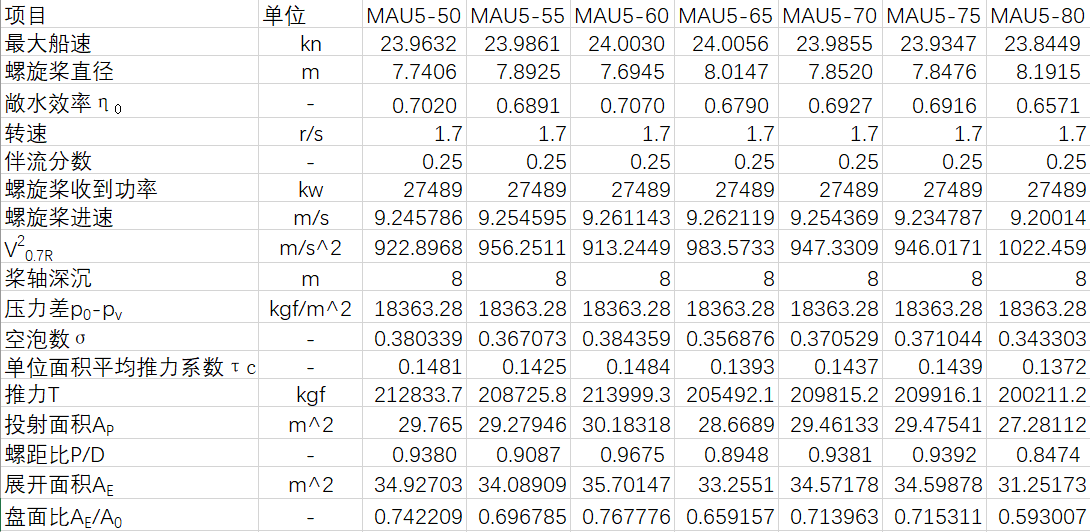
\includegraphics[width=4in]{figure/cavitation_check_sheet.png}
		\caption{Cavitation Check Caculation Sheet}
		\label{fig:cavichecksheet}
	\end{figure}
\end{appendices}
\label{last}  
\end{document}